% radiosynth - From MHD to MHz: thermal free-free (bremsstrahlung) emission, equations and implementation
% Copyright (C) 2026 Soumitra Hazra
% Compile with: pdflatex radiosynth_bremsstrahlung.tex (twice); needs ff_rays.pdf and ff_profiles.pdf
\documentclass[11pt,a4paper]{article}
\usepackage[T1]{fontenc}
\usepackage{lmodern}
\usepackage[margin=2.4cm]{geometry}
\usepackage{amsmath,amssymb,bm}
\usepackage{booktabs,array,longtable}
\usepackage{graphicx}
\usepackage{xcolor}
\usepackage{enumitem}
\usepackage[font=small,labelfont=bf]{caption}
\usepackage[colorlinks=true,linkcolor=blue!50!black,citecolor=blue!50!black,urlcolor=blue!50!black]{hyperref}

\definecolor{accent}{RGB}{31,78,121}
\newcommand{\code}[1]{\texttt{#1}}
\newcommand{\vect}[1]{\bm{#1}}
\newcommand{\dd}{\mathrm{d}}
\newcommand{\kB}{k_\mathrm{B}}
\newcommand{\ncr}{n_\mathrm{cr}}
\newcommand{\rsun}{R_\odot}
\setlist{itemsep=2pt,topsep=4pt}
\setlength{\parskip}{3pt}
\setlength{\emergencystretch}{2.5em}

\newenvironment{incode}{\par\smallskip\noindent\begin{minipage}{\linewidth}\small\color{accent!80!black}\textbf{In the code.}~}{\end{minipage}\par\smallskip}

\hypersetup{pdftitle={Thermal free-free (bremsstrahlung) emission in radiosynth},pdfauthor={Soumitra Hazra}}

\begin{document}

\begin{center}
{\LARGE\bfseries\color{accent} Thermal free--free (bremsstrahlung) emission\\[3pt] in \textsf{radiosynth}\par}
\vspace{0.3cm}
{\large Equations, refractive ray tracing and numerical implementation\par}
\vspace{0.4cm}
{\normalsize Soumitra Hazra\par}
\vspace{0.1cm}
{\small \textsf{radiosynth} 2.2.0 --- \emph{From MHD to MHz} --- November 2026\par}
{\small \url{https://github.com/soumitrahazra/radiosynth}\par}
\end{center}

\begin{abstract}
\noindent This note collects every equation used by \textsf{radiosynth} to compute the thermal
free--free (bremsstrahlung) radio emission of an MHD model of a solar or stellar corona. It
gives the emission and absorption coefficients (constant Gaunt factor or Coulomb logarithm),
the refraction of radio waves in the plasma and the ray equation, the image geometry for an
observer at Earth or at a stellar distance, and the step-by-step numerical integration of the
curved rays: predictor, step control by curvature and by distance to the critical surface,
Boris rotation, parabolic reflection and the recovery of rays that overshoot the critical
surface. It then describes the optically thin and the full radiative transfer, the conversion
to brightness temperature and flux, the comparison with straight lines of sight, the
spherically symmetric (1D) models and the analytic stellar-wind solution used for validation.
Each section names the functions that implement it, so that the equations can be checked
line by line against the code.
\end{abstract}

\tableofcontents

%======================================================================
\section{Overview}
%======================================================================

At metre and decimetre wavelengths the quiet corona shines by thermal free--free emission:
electrons accelerated in the Coulomb field of ions. Its opacity grows as $n_e^2\nu^{-2}T_e^{-3/2}$,
so at low frequencies the corona is optically thick high above the photosphere and the radio
Sun is larger than the optical one, with a brightness temperature close to the coronal
temperature. At the same frequencies the plasma refracts the waves strongly: rays bend away
from dense plasma and are reflected before they reach the \emph{critical density}, where the
plasma frequency equals the observing frequency. Synthetic images of an MHD model therefore
need both the radiative transfer and the curved ray paths.

\textsf{radiosynth} computes a free--free image in four steps:
\begin{enumerate}
  \item set up the image plane and one ray per pixel, starting where the ray enters the model
        (Sect.~\ref{sec:geometry});
  \item trace all rays together through the model with the refractive ray tracer, following
        the algorithm of the BATS-R-US radio-wave imaging module (Benkevitch et al.\ 2010;
        Moschou et al.\ 2018) (Sects.~\ref{sec:refraction}--\ref{sec:step});
  \item along each ray, evaluate the emission and absorption coefficients
        (Sect.~\ref{sec:coeff}) and accumulate the intensity, optically thin or with the full
        transfer (Sect.~\ref{sec:transfer});
  \item convert to brightness temperature and flux (Sect.~\ref{sec:output}).
\end{enumerate}
Straight lines of sight (\code{no\_refraction=True}), 1D symmetric models and stellar
observers use the same machinery (Sects.~\ref{sec:compare}--\ref{sec:stars}).

%======================================================================
\section{Notation, units and constants}\label{sec:notation}
%======================================================================

The code works in SI units. Positions are in coordinate units of the model (solar radii
$\rsun=6.96\times10^8$\,m, or stellar radii $R_\ast$), converted to metres with the grid's
\code{length\_unit} $L_\text{unit}$. In every Gaussian formula $e^2$ stands for
$e^2/4\pi\varepsilon_0$.

\begin{center}
\small
\begin{longtable}{@{}l p{8.6cm} l@{}}
\toprule
Symbol & Meaning & Value / unit \\
\midrule
$\nu$ & observing frequency & Hz \\
$n_e$, $T_e$ & electron density and temperature of the model & m$^{-3}$, K \\
$\nu_p$ & plasma frequency, $\nu_p^2=e^2n_e/(4\pi^2\varepsilon_0m_e)$ & Hz \\
$\ncr$ & critical density, $\nu_p(\ncr)=\nu$: $\ncr=\pi m_e\nu^2/(e^2/4\pi\varepsilon_0)$ & $1.2404\times10^{16}\,(\nu/\text{GHz})^2$\,m$^{-3}$ \\
$\varepsilon$, $\mu$ & dielectric permittivity and refractive index, $\varepsilon=\mu^2=1-n_e/\ncr$ & --- \\
$\vect r$, $\vect v$ & ray position and unit direction, $|\vect v|=1$ & coord.\ units, --- \\
$s$, $\Delta s$ & arc length along the ray and step & coord.\ units \\
$\Delta\ell$ & length of a path segment in metres, $\Delta\ell=\Delta s\,L_\text{unit}$ & m \\
$\kappa_\nu$ & absorption coefficient & m$^{-1}$ \\
$B_\nu$ & source function (Rayleigh--Jeans), $2\nu^2\kB T_e/c^2$ & W\,m$^{-2}$\,Hz$^{-1}$\,sr$^{-1}$ \\
$g$, $G$ & Gaunt factor; Coulomb-logarithm factor of Dulk (1985) & --- \\
$\tau$ & optical depth from the observer & --- \\
$I_\nu$, $T_b$ & specific intensity, brightness temperature & SI, K \\
$F_\nu$ & flux density at the observer ($1\,\text{sfu}=10^{-22}$\,W\,m$^{-2}$\,Hz$^{-1}$) & W\,m$^{-2}$\,Hz$^{-1}$ \\
\bottomrule
\end{longtable}
\end{center}

\begin{incode}
\code{common/constants.py}: \code{E2\_JM} $=e^2/4\pi\varepsilon_0$, \code{R\_SUN},
\code{critical\_density(f)}, \code{plasma\_frequency(ne)}.
\end{incode}

%======================================================================
\section{Emission and absorption coefficients}\label{sec:coeff}
%======================================================================

\subsection{Source function}
The coronal plasma is close to local thermodynamic equilibrium and $h\nu\ll\kB T_e$, so by
Kirchhoff's law the source function is the Rayleigh--Jeans intensity
\begin{equation}
  B_\nu=\frac{2\nu^2\kB T_e}{c^2}.
  \label{eq:rj}
\end{equation}

\subsection{Absorption coefficient with a constant Gaunt factor}
The default coefficient is that of Moschou et al.\ (2018, Eqs.~15--16), used in BATS-R-US,
\begin{equation}
  \kappa_\nu=\frac43\sqrt{\frac{2\pi}{3}}\;
    \frac{\left[e^2/(4\pi\varepsilon_0)\right]^3}{c\,(\kB T_e\,m_e)^{3/2}}\;
    \frac{n_e^2}{\nu^2}\;g,\qquad g=10 .
  \label{eq:kappa}
\end{equation}
Numerically, in SI and in cgs,
\begin{equation}
  \kappa_\nu=1.7720\times10^{-12}\;g\,\frac{n_e^2[\text{m}^{-6}]}{\nu^2T_e^{3/2}}\ \text{m}^{-1}
  \;=\;1.7720\times10^{-2}\;g\,\frac{n_e^2[\text{cm}^{-6}]}{\nu^2T_e^{3/2}}\ \text{cm}^{-1}.
\end{equation}

\subsection{Absorption coefficient with the Coulomb logarithm}
With \code{gaunt="dulk"} the code uses Dulk (1985, Eq.~21),
\begin{equation}
  \kappa_\nu=9.78\times10^{-3}\,\frac{n_e^2}{\nu^2T_e^{3/2}}\,G\ \ \text{cm}^{-1},\qquad
  G=\begin{cases}18.2+\ln T_e^{3/2}-\ln\nu, & T_e<2\times10^5\,\text{K},\\
                 24.5+\ln T_e-\ln\nu, & T_e\ge2\times10^5\,\text{K},\end{cases}
  \label{eq:dulk}
\end{equation}
with $n_e$ in cm$^{-3}$, $G\ge1$, converted to m$^{-1}$. Comparing with Eq.~\eqref{eq:kappa},
the two forms agree for an effective Gaunt factor
\begin{equation}
  g_\text{eff}=\frac{9.78\times10^{-3}}{1.7720\times10^{-2}}\,G=0.552\,G\simeq\frac{\sqrt3}{\pi}\,G .
\end{equation}
In the corona $G\approx16$--21, so $g_\text{eff}\approx9$--11.5 and the constant $g=10$ is a good
approximation (Table~\ref{tab:kappa}).

\begin{table}[ht]
\centering\small
\caption{Absorption coefficient for $n_e=10^9$\,cm$^{-3}$, $T_e=1$\,MK (\code{bremsstrahlung\_coefficients}).}
\label{tab:kappa}
\begin{tabular}{@{}l c c c@{}}
\toprule
$\nu$ & $\kappa$ ($g=10$) [m$^{-1}$] & $\kappa$ (Dulk) [m$^{-1}$] & $g_\text{eff}$ \\
\midrule
80 MHz  & $2.77\times10^{-6}$ & $3.07\times10^{-6}$ & 11.1 \\
300 MHz & $1.97\times10^{-7}$ & $2.04\times10^{-7}$ & 10.4 \\
1 GHz   & $1.77\times10^{-8}$ & $1.72\times10^{-8}$ & 9.7 \\
5 GHz   & $7.09\times10^{-10}$ & $6.25\times10^{-10}$ & 8.8 \\
\bottomrule
\end{tabular}
\end{table}

\subsection{Refractive correction of the absorption}
In a refracting medium the absorption coefficient along the ray is larger by the factor
$1/\mu$, which matters close to the critical layer (Dulk 1985). It is not included in
BATS-R-US and is off by default; with \code{kappa\_over\_mu=True} the code uses
\begin{equation}
  \kappa_\nu\ \to\ \frac{\kappa_\nu}{\mu},\qquad \mu=\sqrt{\max(\varepsilon,10^{-6})} .
\end{equation}

\begin{incode}
\code{bremsstrahlung/emission.py}: \code{bremsstrahlung\_coefficients(ne, te, freq, gaunt)}
returns $(\kappa_\nu,B_\nu)$; $T_e$ is floored at 1\,K. \code{common/emission.py}:
\code{EmissionModel("bremsstrahlung", gaunt=...)} is the callable used by the ray tracer.
The $1/\mu$ factor is applied in \code{trace\_rays} (\code{kappa\_over\_mu}).
\end{incode}

%======================================================================
\section{Refraction in the coronal plasma}\label{sec:refraction}
%======================================================================

\subsection{Refractive index and critical surface}
In an unmagnetised plasma (the magnetic field has a negligible effect on refraction at these
frequencies, $\nu\gg\nu_B$)
\begin{equation}
  \varepsilon=\mu^2=1-\frac{\nu_p^2}{\nu^2}=1-\frac{n_e}{\ncr},\qquad
  \ncr=\frac{\pi m_e\nu^2}{e^2/(4\pi\varepsilon_0)}
  \approx1.24\times10^{14}\left(\frac{\nu}{100\,\text{MHz}}\right)^2\text{m}^{-3}.
  \label{eq:eps}
\end{equation}
Waves cannot propagate where $n_e>\ncr$ ($\varepsilon<0$). The critical surface $n_e=\ncr$ acts
as a mirror, and most rays are reflected well above it. Table~\ref{tab:levels} gives its height in
the Newkirk (1961) corona, $n_e=4.2\times10^4\times10^{4.32/r}$\,cm$^{-3}$.

\begin{table}[ht]
\centering\small
\caption{Critical density and its height in the Newkirk corona; $r(\ncr/4)$ is where
$\nu_p=\nu/2$ (the level of harmonic plasma emission, for reference).}
\label{tab:levels}
\begin{tabular}{@{}l c c c@{}}
\toprule
$\nu$ & $\ncr$ [cm$^{-3}$] & $r(\ncr)$ [$\rsun$] & $r(\ncr/4)$ [$\rsun$] \\
\midrule
30 MHz  & $1.12\times10^{7}$ & 1.78 & 2.37 \\
80 MHz  & $7.94\times10^{7}$ & 1.32 & 1.62 \\
150 MHz & $2.79\times10^{8}$ & 1.13 & 1.34 \\
300 MHz & $1.12\times10^{9}$ & below the photosphere & 1.13 \\
1 GHz   & $1.24\times10^{10}$ & below the photosphere & below \\
\bottomrule
\end{tabular}
\end{table}

\subsection{Ray equation}
From Fermat's principle, $\delta\!\int\mu\,\dd s=0$, with the arc length $s$ as parameter and
$\vect v=\dd\vect r/\dd s$ (Benkevitch et al.\ 2010; Moschou et al.\ 2018, Eq.~7),
\begin{equation}
  \frac{\dd\vect r}{\dd s}=\vect v,\qquad
  \frac{\dd\vect v}{\dd s}=\vect v\times\left(\frac{\nabla\mu}{\mu}\times\vect v\right)
   =\frac{\nabla\mu}{\mu}-\vect v\left(\vect v\cdot\frac{\nabla\mu}{\mu}\right),\qquad
  \frac{\nabla\mu}{\mu}=\frac{\nabla\varepsilon}{2\varepsilon},\quad
  \nabla\varepsilon=-\frac{\nabla n_e}{\ncr}.
  \label{eq:ray}
\end{equation}
The direction only rotates, about the vector $\vect\Omega=(\nabla\mu/\mu)\times\vect v$, like the
velocity of a charged particle in a magnetic field; this is why the Boris particle pusher can be
used (Sect.~\ref{sec:boris}). The curvature of the ray is
\begin{equation}
  \kappa_\text{c}=|\vect\Omega|=\frac{|\nabla_\perp\varepsilon|}{2\varepsilon},\qquad
  |\nabla_\perp\varepsilon|^2=|\nabla\varepsilon|^2-(\nabla\varepsilon\cdot\vect v)^2 .
  \label{eq:curv}
\end{equation}

\subsection{Spherically symmetric corona: Bouguer's invariant}
If $n_e=n_e(r)$, Eq.~\eqref{eq:ray} conserves the quantity (Bouguer's rule)
\begin{equation}
  \mu(r)\,r\sin\psi=b,
  \label{eq:bouguer}
\end{equation}
where $\psi$ is the angle between $\vect v$ and $\vect r$, and $b$ is the impact parameter of the
ray far from the Sun ($\mu=1$). The ray turns at the radius $r_0$ where $\psi=90^\circ$,
\begin{equation}
  \mu(r_0)\,r_0=b,
\end{equation}
above the critical surface for any $b>0$. Fig.~\ref{fig:rays} shows rays at 80\,MHz computed by
the code; Eq.~\eqref{eq:bouguer} is used to test the integration (Sect.~\ref{sec:validation}).

\begin{figure}[ht]
\centering
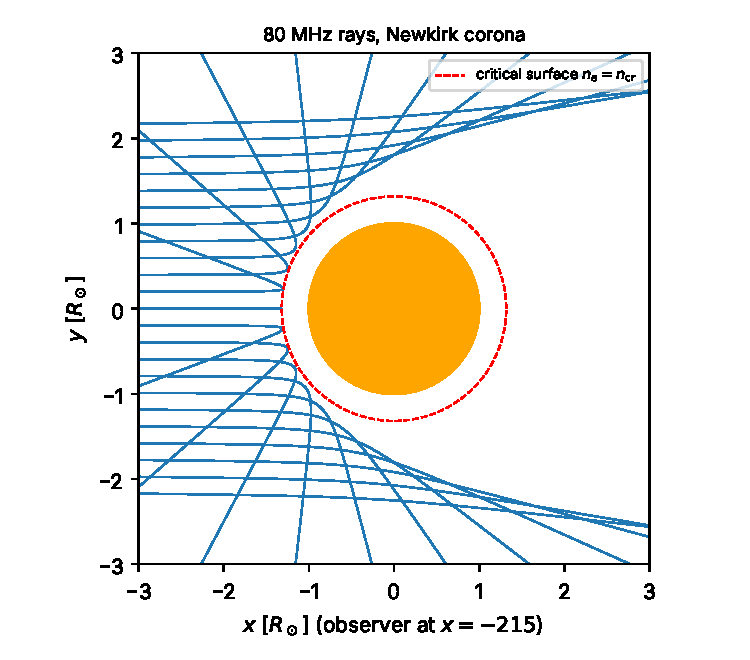
\includegraphics[width=0.56\textwidth]{ff_rays.pdf}
\caption{Ray paths at 80\,MHz through a spherically symmetric Newkirk corona, computed with
\code{rs.trace\_paths}. The rays come from the observer on the left, bend away from the dense
plasma and are reflected above the critical surface (red, $r=1.32\,\rsun$).}
\label{fig:rays}
\end{figure}

%======================================================================
\section{Image geometry}\label{sec:geometry}
%======================================================================

\subsection{Image plane and rays}
The observer is at $\vect O$ (default $(-215,0,0)\,\rsun$, the Earth on the $-x$ axis). With the
unit vectors
\begin{equation}
  \hat{\vect n}=\frac{\vect O}{|\vect O|},\qquad
  \hat{\vect\tau}=\frac{\hat{\vect u}\times\hat{\vect n}}{|\hat{\vect u}\times\hat{\vect n}|},\qquad
  \hat{\vect\xi}=\hat{\vect n}\times\hat{\vect\tau},
\end{equation}
where $\hat{\vect u}$ is the ``up'' direction (default $\hat z$), the image plane passes through
the centre of the Sun. The pixel centres are
\begin{equation}
  X_i=-\tfrac12X_\text{size}+\left(i+\tfrac12\right)\Delta X,\qquad
  Y_j=-\tfrac12Y_\text{size}+\left(j+\tfrac12\right)\Delta Y,\qquad
  \vect P_{ij}=X_i\hat{\vect\tau}+Y_j\hat{\vect\xi},
\end{equation}
($i=0\ldots n_x-1$, $\Delta X=X_\text{size}/n_x$) and the initial ray directions are
\begin{equation}
  \vect v_0=\frac{\vect P_{ij}-\vect O}{|\vect P_{ij}-\vect O|}.
\end{equation}

\subsection{Integration sphere and starting point}
The rays are followed inside the integration sphere of radius
\begin{equation}
  r_\text{int}=\left\lceil\max\!\left(\sqrt{(X_\text{size}/2)^2+(Y_\text{size}/2)^2}+1,\ 5\right)\right\rceil
\end{equation}
(as in BATS-R-US; the keyword \code{r\_integration} overrides it). Each ray starts at the
\emph{later} of two points: where it enters the integration sphere and where it enters the model
domain. The vacuum in front contributes nothing, and this matters when the model box is smaller
than the sphere. Rays that miss the domain are flagged as \code{MISSED}.

\subsection{Distant observers}
For a star at distance $D$ (\code{distance\_pc}) the rays are parallel to $-\hat{\vect n}$. The
ray of pixel $(i,j)$ passes through $\vect P_{ij}$ and starts outside the model at
$\vect P_{ij}+R_\text{far}\hat{\vect n}$ with $R_\text{far}=4\max(r_\text{int},r_\text{outer},
\tfrac12\text{diagonal})$. The distance in coordinate units is
$D=d_\text{pc}\times3.0857\times10^{16}\,\text{m}/L_\text{unit}$.

\begin{incode}
\code{common/image.py}: \code{image\_geometry} ($\hat{\vect n},\hat{\vect\tau},\hat{\vect\xi}$,
pixel centres, directions; \code{parallel=True} for stars), \code{start\_points} (first point inside
both the sphere and the domain, status \code{MISSED}); \code{make\_radio\_image} sets
$r_\text{int}$ and $R_\text{far}$.
\end{incode}

%======================================================================
\section{Numerical integration of the rays}\label{sec:step}
%======================================================================

All active rays advance together: every quantity below is an array over the rays, and the
decisions are boolean masks. The model supplies, at any point, $n_e$, $\nabla n_e$ (computed once on
the grid with second-order finite differences and interpolated trilinearly), $T_e$ and the local
cell size $\Delta_\text{cell}$. One step from $(\vect r_0,\vect v_0)$ with step $\Delta s$ consists
of the following.

\subsection{Predictor and termination tests}
\begin{equation}
  \vect r_{1/2}=\vect r_0+\vect v_0\,\frac{\Delta s}{2},
\end{equation}
where $n_e$, $\nabla n_e$, $T_e$ and $\Delta_\text{cell}$ are sampled. The ray stops if
\begin{itemize}
  \item $|\vect r_{1/2}|<r_\text{body}$ --- it has reached the photosphere (\code{HIT\_BODY}); the
        remaining straight piece to the surface, of length
        $t=-b-\sqrt{b^2-c}$ with $b=\vect r_0\cdot\vect v_0$, $c=r_0^2-r_\text{body}^2$ (limited to
        $[0,\Delta s]$), is still integrated with $n_e$ capped at $\ncr$;
  \item it has left the domain or the integration sphere (\code{ESCAPED});
  \item $n_e(\vect r_{1/2})\ge\ncr$ (\code{OVERDENSE}; recovered in the default mode, below).
\end{itemize}

\subsection{Permittivity}
\begin{equation}
  \varepsilon_{1/2}=1-\frac{n_e}{\ncr},\qquad
  \nabla\varepsilon=-\frac{\nabla n_e}{\ncr},\qquad
  \varepsilon_0=\varepsilon_{1/2}-(\nabla\varepsilon\cdot\vect v_0)\,\frac{\Delta s}{2},
  \label{eq:eps0}
\end{equation}
the last being the back-extrapolated permittivity at the start of the step (Benkevitch et al.\
2010, Eq.~34). If $\varepsilon_0\le0$ the ray has crossed the critical surface (\code{NEG\_EPS}).

\subsection{Recovery of rays that cross the critical surface}
In the default mode such rays are not discarded (Benkevitch et al.\ 2010, Sect.~5.2; Moschou et
al.\ 2018, Sect.~2.2):
\begin{enumerate}
  \item if $\Delta s\ge4\Delta s_\text{min}$, the step is retried from the same point with
        $\Delta s/4$;
  \item otherwise, if the ray moves into the gradient ($\nabla\varepsilon\cdot\vect v<0$), its direction
        is reflected specularly (Snell's law),
        \begin{equation}
          \vect v\ \leftarrow\ \vect v-2(\vect v\cdot\hat{\vect g})\,\hat{\vect g},\qquad
          \hat{\vect g}=\frac{\nabla\varepsilon}{|\nabla\varepsilon|},
        \end{equation}
        the step is reset to at least $\Delta s_\text{step,min}$ and the steep flag is cleared.
\end{enumerate}
$\Delta s_\text{min}=10^{-6}$ (\code{min\_ds}) and $\Delta s_\text{step,min}=10^{-2}$
(\code{step\_min}) in coordinate units.

\subsection{Precision control}\label{sec:check}
For rays that are not marked \emph{steep}, two tests decide whether the step is accepted.

\paragraph{(a) Curvature.} The squared turning angle over half a step is, from Eq.~\eqref{eq:curv}
with $\varepsilon\to\varepsilon_0$,
\begin{equation}
  \left(\kappa_\text{c}\frac{\Delta s}{2}\right)^2=\left(\frac{\Delta s}{4\varepsilon_0}\right)^2
  \left(|\nabla\varepsilon|^2-(\nabla\varepsilon\cdot\vect v_0)^2\right).
\end{equation}
If it is $\ge\text{Tol}^2$ (\code{tolerance} $=10^{-2}$, about 50 steps per radian), the step is
redone with
\begin{equation}
  \Delta s\ \leftarrow\ \frac{0.99\,\Delta s}{2\sqrt{(\kappa_\text{c}\Delta s/2)^2/\text{Tol}^2}},
\end{equation}
not below $\Delta s_\text{min}$ in the default mode.

\paragraph{(b) Approach to the critical surface.} If a linear prediction puts $\varepsilon=0$
within about 1.5 steps (Benkevitch et al.\ 2010, Eq.~33),
\begin{equation}
  3\,(\nabla\varepsilon\cdot\vect v_0)\,\frac{\Delta s}{2}\le-\varepsilon_0,
  \label{eq:steep}
\end{equation}
the ray is marked steep, the distance to the critical surface
$d_\text{cr}=\varepsilon_0/|\nabla\varepsilon|$ is stored, and the step is redone with
$\Delta s\leftarrow\max(\tfrac12\text{Tol}\,d_\text{cr},\ \Delta s_\text{step,min})$.

In both cases the ray stays at $\vect r_0$ and tries again in the next iteration.

\subsection{Advance: Boris step}\label{sec:boris}
For an accepted step the direction is rotated with the Boris (CYLRAD) scheme (Benkevitch et al.\
2010, Eq.~24). With
\begin{equation}
  \vect a=\frac{\nabla\varepsilon}{2\varepsilon_{1/2}}\,\frac{\Delta s}{2}=\frac{\nabla\mu}{\mu}\frac{\Delta s}{2},
\end{equation}
\begin{align}
  \vect\Omega_0&=\vect a\times\vect v_0, & \vect v'&=\vect v_0+\vect v_0\times\vect\Omega_0,\nonumber\\
  \vect\Omega_{1/2}&=\vect a\times\vect v', & \vect v''&=\vect v_0+\vect v_0\times\vect\Omega_{1/2},\nonumber\\
  \vect v_1&=\vect v_0+\frac{2}{1+\Omega_{1/2}^2}\,\vect v''\times\vect\Omega_{1/2}, &
  \vect r_1&=\vect r_{1/2}+\vect v_1\frac{\Delta s}{2}.
\end{align}
The rotation keeps $|\vect v|=1$ exactly and is second-order accurate. The segment length is
$\Delta s$.

\subsection{Advance: parabolic switch at the critical surface}\label{sec:parab}
For rays that satisfy Eq.~\eqref{eq:steep} even after the step was reduced, the ray is close to
its turning point. If $\nabla\varepsilon$ is constant over the step the path is a parabola. With
$L=1/|\nabla\varepsilon|$ and $\alpha$ the angle between $\vect v_0$ and $-\nabla\varepsilon$,
\begin{align}
  L\cos\alpha&=-\frac{\nabla\varepsilon\cdot\vect v_0}{|\nabla\varepsilon|^2}, &
  \vect v_\parallel&=-L\cos\alpha\,\nabla\varepsilon,\nonumber\\
  \vect v_1&=\vect v_0-2\vect v_\parallel, &
  \Delta\vect r_\perp&=4\,(\vect v_0-\vect v_\parallel)\,L\cos\alpha\,\varepsilon_0,\nonumber\\
  \vect r_1&=\vect r_0+\Delta\vect r_\perp, &
  \Delta\vect r_\parallel&=\varepsilon_0\,(L\cos\alpha)^2\,\nabla\varepsilon,
\end{align}
and the emission of the arc is counted over the length
\begin{equation}
  \Delta s_\text{arc}=\sqrt{|2\Delta\vect r_\parallel|^2+|\Delta\vect r_\perp|^2}.
\end{equation}
The ray jumps to the symmetric point on the other branch of the parabola, with its normal
velocity component reversed.

\subsection{Clipping at the photosphere}
If the new point $\vect r_1$ lies inside $r_\text{body}$, only the fraction
$t\in[0,1]$ of the segment outside the body is counted, from the first root of
$|\vect r_0+t(\vect r_1-\vect r_0)|=r_\text{body}$; the ray ends (\code{HIT\_BODY}).

\subsection{Step regrowth}
After an accepted step, for gentle rays and for steep rays that have moved away from the critical
surface ($\varepsilon_0>d_\text{cr}|\nabla\varepsilon|$), the steep flag is cleared and
\begin{equation}
  \Delta s\ \leftarrow\ \max\!\left(2-\frac{\Delta s}{\Delta s_\text{new}},\,1\right)
     \min(\Delta s_\text{new},\Delta s),\qquad \Delta s_\text{new}=f_\text{step}\,\Delta_\text{cell},
\end{equation}
which roughly doubles small steps and saturates smoothly at $\Delta s_\text{new}$
($f_\text{step}=$ \code{step\_factor}, default 1). The first step of a ray is
$f_\text{step}\Delta_\text{cell}$ at its starting point (or \code{ds\_init}).

\subsection{The original BATS-R-US logic}\label{sec:strict}
With \code{strict\_batsrus=True} the code reproduces the step logic of the BATS-R-US module
exactly. It differs from the default in two places:
\begin{enumerate}
  \item BATS-R-US also uses the parabolic switch whenever $\Delta s<\Delta s_\text{step,min}$
        and $\nabla\varepsilon\cdot\vect v<0$. This condition is reached after the curvature
        control has shrunk the step, so it fires on rays far from the critical surface, which then
        jump along a long, wrong parabola. The default mode uses the switch only under
        Eq.~\eqref{eq:steep}.
  \item BATS-R-US discards rays that land in over-dense plasma or have $\varepsilon_0\le0$; the
        default mode recovers them (step back and Snell reflection).
\end{enumerate}
The default mode also has the lower bound $\Delta s_\text{min}$ in the curvature control.

\subsection{Ray status}
Every ray ends with one of the codes \code{ESCAPED} (left the domain or the sphere),
\code{HIT\_BODY}, \code{OVERDENSE}, \code{NEG\_EPS} (the last two mainly in strict mode or without
refraction; in the default mode only rays that cannot be reflected end this way), \code{OPAQUE} ($\tau>\tau_\text{max}$, full transfer), \code{MAX\_STEPS} (safety limit,
200\,000 iterations) or \code{MISSED}; they are stored per pixel in \code{img.status}.

\begin{incode}
\code{common/raytrace.py}, function \code{trace\_rays}, one subroutine per stage:
\code{\_predictor}, \code{\_terminations}, \code{\_integrate\_to\_body}, \code{\_dielectric}
(Eq.~\ref{eq:eps0}), \code{\_snell\_fallback}, \code{\_check\_step} (Sect.~\ref{sec:check}),
\code{\_advance} with \code{\_boris\_step} and \code{\_parabolic\_step}, \code{\_clip\_at\_body},
\code{\_add\_emission} (Sect.~\ref{sec:transfer}) and \code{\_new\_step\_size}. Keywords:
\code{tolerance}, \code{step\_min}, \code{min\_ds}, \code{step\_factor}, \code{ds\_init},
\code{strict\_batsrus}, \code{max\_steps}. The gradient $\nabla n_e$ is computed in
\code{common/grid.py} (\code{np.gradient}, second order).
\end{incode}

%======================================================================
\section{Radiative transfer along the ray}\label{sec:transfer}
%======================================================================

For each accepted segment, $\kappa_\nu$ and $B_\nu$ are evaluated at the mid-point $\vect r_{1/2}$
and the segment length in metres is $\Delta\ell=\Delta s\,f_\text{clip}\,L_\text{unit}$ (with the arc
length for a parabolic step and the clipping fraction at the photosphere).

\subsection{Optically thin (default, as in BATS-R-US)}
\begin{equation}
  I_\nu=\sum_\text{segments}\kappa_\nu B_\nu\,\Delta\ell .
  \label{eq:thin}
\end{equation}
This is what BATS-R-US and Moschou et al.\ (2018, Eq.~14) use. It neglects absorption, so in the
dense low corona it can give $T_b>T_e$ (Fig.~\ref{fig:profiles}, right).

\subsection{Full transfer}
With \code{transfer="full"} the code solves $\dd I/\dd s=\kappa(B-I)$ exactly for constant
$\kappa$ and $B$ on each segment, integrating from the observer into the medium:
\begin{equation}
  I_\nu=\sum_\text{segments}B_\nu\,e^{-\tau}\left(1-e^{-\Delta\tau}\right),\qquad
  \Delta\tau=\kappa_\nu\Delta\ell,\qquad \tau\leftarrow\tau+\Delta\tau,
  \label{eq:full}
\end{equation}
where $\tau$ is the optical depth between the observer and the start of the segment
($1-e^{-x}$ is evaluated as \code{-expm1(-x)}). This gives $T_b\le T_e$ in isothermal plasma and the
optical depth $\tau$ of every pixel. Once $\tau>\tau_\text{max}$ (default 30,
$e^{-30}\approx10^{-13}$) nothing more can be seen and the ray stops (\code{OPAQUE}). The full
transfer is recommended for physically meaningful brightness temperatures below about 1\,GHz.

Neither mode adds emission from the photosphere behind a ray that reaches $r_\text{body}$.

\begin{figure}[ht]
\centering
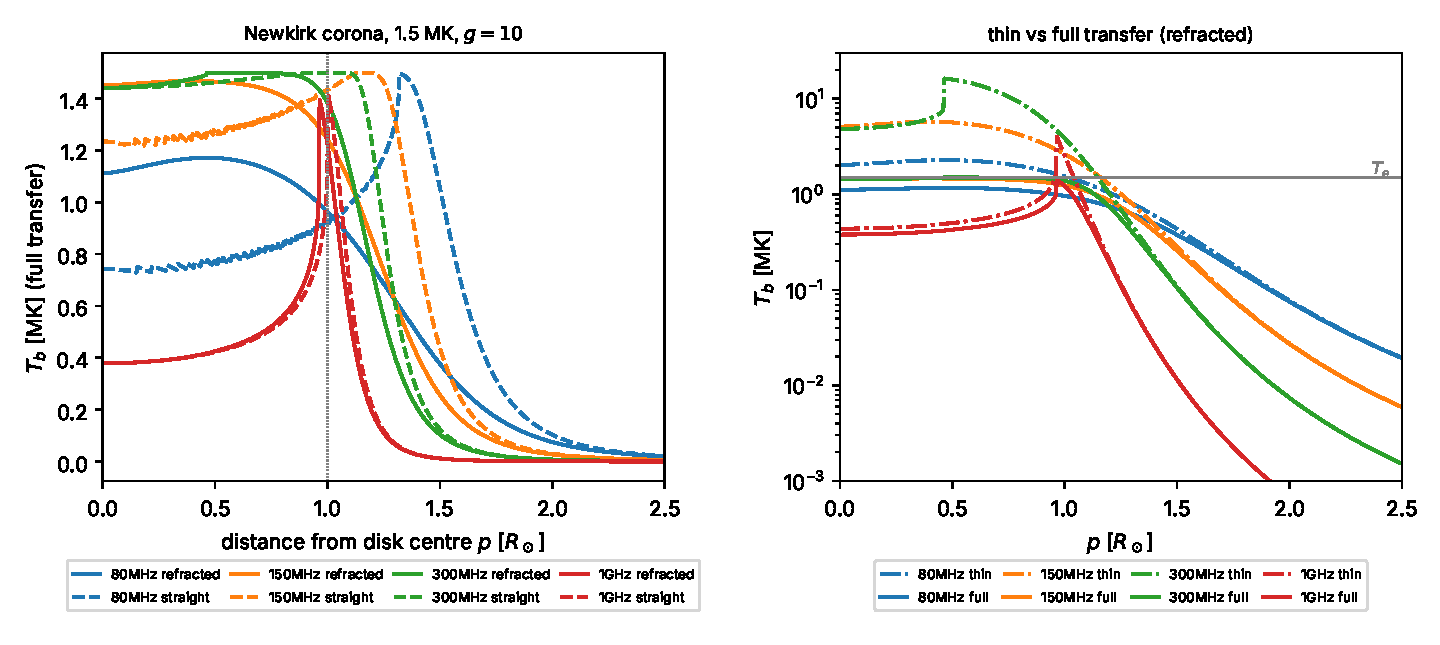
\includegraphics[width=\textwidth]{ff_profiles.pdf}
\caption{Brightness temperature against distance from the disk centre for a spherically
symmetric Newkirk corona with $T_e=1.5$\,MK and $g=10$, computed with
\code{rs.make\_symmetric\_image}. Left: full transfer, refracted rays (solid) and straight lines
of sight (dashed). At 80 and 150\,MHz refraction makes the radio Sun smaller (the
limb falls off closer to the disk; the fluxes are 3.1 and 11.7\,sfu instead of 4.1 and 14.4\,sfu)
but its centre brighter: straight lines stop at the critical surface after an optical depth below
one, while refracted rays turn above it and travel longer through the dense plasma. At 1\,GHz the
two agree. Right: refracted rays, thin (dash-dotted) and full (solid) transfer; the thin
sum exceeds $T_e$ where the corona is optically thick.}
\label{fig:profiles}
\end{figure}

\begin{incode}
\code{common/raytrace.py}: \code{\_add\_emission(intensity, tau, idx, kappa, B, dl, transfer)}
(Eqs.~\ref{eq:thin} and \ref{eq:full}); \code{tau\_max} in \code{trace\_rays}.
\end{incode}

%======================================================================
\section{Brightness temperature and flux}\label{sec:output}
%======================================================================

\begin{equation}
  T_b=\frac{c^2}{2\kB\nu^2}\,I_\nu,\qquad
  F_\nu=\sum_\text{pixels}I_\nu\,\Delta\Omega,\qquad
  \Delta\Omega=\frac{\Delta X\,\Delta Y}{D^2},
\end{equation}
with $D=|\vect O|$ (or the stellar distance) and all lengths in the same unit. The flux is also
given in sfu ($10^{-22}$\,W\,m$^{-2}$\,Hz$^{-1}$) and Jy ($10^{-26}$).

\begin{incode}
\code{common/image.py}, class \code{RadioImage}: \code{intensity}, \code{tau}, \code{status},
\code{brightness\_temperature}, \code{pixel\_solid\_angle}, \code{flux\_density}, \code{summary()},
\code{save\_npz}, \code{save\_fits}, \code{plot}.
\end{incode}

%======================================================================
\section{Refracted rays versus straight lines of sight}\label{sec:compare}
%======================================================================

With \code{no\_refraction=True} the rays are straight lines: the step control and the reflection
are skipped, the direction is never changed and the step regrows to the cell size. The rays still
stop where $n_e\ge\ncr$, since the waves cannot propagate there. The difference between the two
images measures the effect of refraction (Fig.~\ref{fig:profiles}, left). At low frequencies the
radio Sun is smaller with refraction, because rays passing near the limb are bent away from the
dense plasma and see less of it. Near the disk centre the opposite can happen: a straight line
stops at the critical surface, possibly before it becomes optically thick, whereas a refracted ray
turns above the critical surface and accumulates more optical depth near its turning point, so
the centre can be brighter with refraction. At high frequencies, where $n_e\ll\ncr$, the two
agree.

\code{rs.compare\_refraction(grid, freqs, ...)} computes both images with identical options and
returns a dictionary with the two images (\code{refracted}, \code{straight}), the flux ratio
refracted/straight per frequency (\code{flux\_ratio}) and, if \code{path} is given, a figure of
both images and their ratio
(\code{--compare-refraction} on the command line).

%======================================================================
\section{Spherically symmetric (1D) models}\label{sec:sym}
%======================================================================

A 1D model gives $n_e(r)$ and $T_e(r)$ (\code{rs.grid\_from\_profile}, \code{rs.read\_profile}, or
1D spherical PLUTO output). Its image depends only on the distance $p$ from the disk centre, and
the problem is symmetric about the observer--Sun axis also with refraction and for an observer at
finite distance. \code{rs.make\_symmetric\_image} therefore traces a single row of rays,
$p_k=k\,\Delta p$, $k=0\ldots n_p$ ($\Delta p=p_\text{max}/n_p$, default $n_p=1000$), rotates the
result into a 2D image, and integrates the flux over the whole disk $p\le p_\text{max}$ exactly:
\begin{equation}
  F_\nu=\frac{2\pi}{D^2}\int_0^{p_\text{max}}I_\nu(p)\,p\,\dd p
\end{equation}
(trapezoidal rule). It also returns the profiles $I_\nu(p)$ and $T_b(p)$
(Fig.~\ref{fig:profiles}).

\begin{incode}
\code{common/symmetric.py}: \code{grid\_from\_profile}, \code{read\_profile},
\code{make\_symmetric\_image} (one row of $2n_p+1$ rays through the centre, rotation with
\code{\_rotate}, profile flux), \code{plot\_profile}.
\end{incode}

%======================================================================
\section{Stars and the analytic wind}\label{sec:stars}
%======================================================================

For a star, coordinates are in stellar radii ($L_\text{unit}=R_\ast$), the observer is at a
distance in parsec and the rays are parallel (Sect.~\ref{sec:geometry}). The code is validated
against the classic isothermal, fully ionised wind $n_e=n_0(r_0/r)^2$ with constant $g$ (Wright \&
Barlow 1975; Panagia \& Felli 1975). Writing $\kappa=\kappa_1n_e^2$, the optical depth along a
straight line at impact parameter $p$ is
\begin{equation}
  \tau(p)=\kappa_1n_0^2r_0^4\int_{-\infty}^{\infty}\frac{\dd l}{(p^2+l^2)^2}
        =\frac{a}{p^3},\qquad a=\frac{\pi}{2}\,\kappa_1n_0^2r_0^4 .
\end{equation}
The flux of the infinite wind (neglecting the stellar disk) is
\begin{equation}
  F_\nu=\frac{2\pi B_\nu}{D^2}\int_0^\infty\left(1-e^{-a/p^3}\right)p\,\dd p
       =\frac{2\pi B_\nu}{D^2}\,\frac{a^{2/3}}{3}\int_0^\infty\left(1-e^{-x}\right)x^{-5/3}\dd x
       =\frac{\pi\,\Gamma(1/3)\,B_\nu\,a^{2/3}}{D^2},
\end{equation}
using $x=a/p^3$ and $\int_0^\infty(1-e^{-x})x^{-5/3}\dd x=\tfrac32\Gamma(\tfrac13)$ (integration
by parts). Since $B_\nu\propto\nu^2$ and $a\propto\nu^{-2}$, $F_\nu\propto\nu^{2/3}$ (the classic
$\nu^{0.6}$ once the weak frequency dependence of the Gaunt factor is included). For $p<r_0$ the
line stops at the stellar surface and the code integrates the front half numerically.

\begin{incode}
\code{bremsstrahlung/wind.py}: \code{wind\_optical\_depth}, \code{wind\_flux\_density};
\code{common/stellar.py}: stellar observers, spectra, spectral indices.
\end{incode}

%======================================================================
\section{Magnetised free--free emission}\label{sec:mag}
%======================================================================

In a magnetic field the two magneto-ionic modes have different free--free absorption,
\begin{equation}
  \kappa_\sigma=\frac{\kappa_\nu}{(1+\sigma q)^2},\qquad q=\min(Y|\cos\theta|,0.9),\qquad
  Y=\frac{\nu_B}{\nu},\quad \sigma=+1\ (\text{o}),\,-1\ (\text{x}),
\end{equation}
each with half of $B_\nu$, which gives $V/I=2q/(1+q^2)\simeq2Y|\cos\theta|$ for a thin source. This
polarised form is used by the gyroresonance and combined images, along straight rays (see the
companion note on gyroresonance emission); the refractive images described here are unpolarised.

%======================================================================
\section{Assumptions and range of validity}\label{sec:limits}
%======================================================================

\begin{enumerate}
  \item \textbf{Thermal, Rayleigh--Jeans emission}, $h\nu\ll\kB T_e$, with a constant or
        Coulomb-logarithm Gaunt factor; free--free emission of electrons on ions only.
  \item \textbf{Geometrical optics.} The model must resolve the density scale height near the
        critical layer; with cells of 0.025--0.05\,$\rsun$ the accuracy is about 1\,\%.
  \item \textbf{Refraction in an unmagnetised plasma}; no scattering by density
        fluctuations, which matters below about 200\,MHz (Moschou et al.\ 2018), and no plasma
        (coherent) emission.
  \item \textbf{No emission from the photosphere or chromosphere} behind rays that reach
        $r_\text{body}$; above $\sim1$\,GHz the model must contain the chromosphere and transition
        region for realistic disk brightness.
  \item \textbf{Thin transfer} is valid only where $\tau\ll1$; use the full transfer otherwise.
\end{enumerate}

%======================================================================
\section{Validation}\label{sec:validation}
%======================================================================

The scripts \code{tests/validate.py}, \code{tests/test\_stellar.py},
\code{tests/test\_symmetric.py} and \code{tests/test\_refraction\_compare.py} check the
implementation (Newkirk corona, $T_e=1.5$\,MK, $0.025\,\rsun$ grid unless stated otherwise):

\begin{center}
\small
\begin{tabular}{@{}p{10.6cm} l@{}}
\toprule
Test & Result \\
\midrule
Bouguer invariant $\mu r\sin\psi$ conserved along rays (80\,MHz) & 1.2\,\% max.\ deviation \\
Turning radius vs.\ analytic $\mu(r_0)r_0=b$ & $4\times10^{-4}\,\rsun$ \\
Exit direction vs.\ \code{scipy solve\_ivp} of Eq.~\eqref{eq:ray} (150\,MHz) & $\le0.3^\circ$ \\
Straight-ray intensity vs.\ quadrature (1, 17\,GHz) & $\le0.9\,\%$ \\
Full transfer: $T_b\le T_e$ & yes \\
Flux vs.\ step size (\code{step\_factor} 1 $\to$ 0.25, 150\,MHz) & $3\times10^{-4}$ \\
Stellar wind: $\tau$ per pixel vs.\ analytic & 0.08\,\% \\
Stellar wind: flux vs.\ exact; analytic $F_\nu$ vs.\ quadrature & 0.02\,\%; $10^{-7}$ \\
Coordinates in $\rsun$ vs.\ $R_\ast$ & identical \\
Symmetric image (one row of rays) vs.\ full 2D image: flux; $T_b$ along a row & $2\times10^{-4}$; $3\times10^{-4}$ \\
1D profile grid vs.\ 3D Cartesian grid of the same corona & 0.02--2\,\% \\
Optically thick wind from a text table: profile flux vs.\ exact integral & $2\times10^{-4}$ \\
\code{compare\_refraction} vs.\ separate runs; 17\,GHz refracted/straight flux & identical; $1-2\times10^{-4}$ \\
\bottomrule
\end{tabular}
\end{center}

%======================================================================
\section{Using it}\label{sec:use}
%======================================================================

\begin{small}
\begin{verbatim}
import radiosynth as rs
grid = rs.load_pluto("out/", nout=27)        # or rs.load_mhd("box.dat")
img = rs.make_radio_image(grid, "80MHz, 150MHz, 300MHz", x_size=6, y_size=6,
                          nx=256, ny=256, transfer="full", gaunt=10.0)
img.plot("tb"); print(img.summary())
cmp = rs.compare_refraction(grid, "80MHz", transfer="full", path="refraction.png")
print(cmp["flux_ratio"])     # cmp["refracted"], cmp["straight"] are images
\end{verbatim}
\end{small}
or, from the command line,
\begin{small}
\begin{verbatim}
python -m radiosynth out/ --freq "80MHz, 150MHz" --size 6 6 --npix 256 256 \
       --transfer full --plot --out quiet_sun
\end{verbatim}
\end{small}

\begin{center}
\small
\begin{tabular}{@{}l l@{}}
\toprule
Keyword of \code{make\_radio\_image} & Quantity in this note \\
\midrule
\code{gaunt} (number or \code{"dulk"}; default 10) & $g$ or $G$, Sect.~\ref{sec:coeff} \\
\code{transfer} (\code{"thin"}, \code{"full"}) & Eq.~\eqref{eq:thin} or \eqref{eq:full} \\
\code{no\_refraction} & straight lines, Sect.~\ref{sec:compare} \\
\code{kappa\_over\_mu} & $\kappa/\mu$ \\
\code{tau\_max} & $\tau_\text{max}$ (full transfer) \\
\code{tolerance}, \code{step\_min}, \code{min\_ds} & Tol, $\Delta s_\text{step,min}$, $\Delta s_\text{min}$ \\
\code{step\_factor}, \code{ds\_init} & $f_\text{step}$, first step \\
\code{strict\_batsrus} & Sect.~\ref{sec:strict} \\
\code{observer}, \code{up}, \code{x\_size}, \code{nx}, \code{r\_integration}, \code{distance\_pc} & Sect.~\ref{sec:geometry} \\
\code{n\_workers} & parallel processes over the rays \\
\bottomrule
\end{tabular}
\end{center}

%======================================================================
\section*{References}
\addcontentsline{toc}{section}{References}
%======================================================================
\begin{small}
\begin{itemize}[leftmargin=1.2em,itemsep=1pt]
\item Benkevitch, L., Sokolov, I., Oberoi, D., \& Zurbuchen, T.\ 2010, ApJ 725, 447 ---
      algorithm for computation of radio images of the Sun.
\item Boris, J.\ P.\ 1970, Proc.\ 4th Conf.\ Numerical Simulation of Plasmas.
\item Dulk, G.\ A.\ 1985, ARA\&A 23, 169 --- radio emission from the Sun and stars.
\item Moschou, S.-P., Sokolov, I., Cohen, O., et al.\ 2018, ApJ 867, 51 --- synthetic radio
      imaging for quiescent and CME-flare scenarios.
\item Newkirk, G.\ 1961, ApJ 133, 983.
\item Panagia, N., \& Felli, M.\ 1975, A\&A 39, 1.
\item Wright, A.\ E., \& Barlow, M.\ J.\ 1975, MNRAS 170, 41.
\end{itemize}
\end{small}

\end{document}
